%% TITLE	Physiological Fluid Mechanics, Summary 7

%% AUTHOR	BINGHUAN W LI (Dept. Chemical Eng/Bio Eng, Imperial)
%%          PETER Y XIE (Dept. Mech Eng, Stanford)

%% compiled in XeLaTeX with Tex Live version 2023.

%% This work is licensed under a Creative Commons Attribution-NonCommercial 4.0 International License.

%=====================================================

\documentclass[a4paper]{article}
\def\NotesType{1}
\def\summaryNo{7}
\def\finalise{1}
%% TITLE	Physiological Fluid Mechanics, configuration

%% DATE		- Nov 19, 2023     create

%% AUTHOR	BINGHUAN W LI (Dept. Chemical Eng/Bio Eng, Imperial)
%%          PETER Y XIE (Dept. Mech Eng, Stanford)

%% compiled in XeLaTeX with Tex Live version 2023.

%% This work is licensed under a Creative Commons Attribution-NonCommercial 4.0 International License.

\usepackage[sfdefault]{arimo}
\usepackage[left=1.5cm, right=1.5cm, top=2cm, bottom=1.5cm]{geometry}
\usepackage{amsmath, amsfonts, amssymb, cancel}
\usepackage{unicode-math}
\setmathfont
    [    Extension = .otf,
         BoldFont = XITSMath-Bold,
    ]{XITSMath-Regular}

% % \DeclareMathSizes{10}{12}{10}{9}

% \usepackage{siunitx}
\usepackage{enumitem}
\usepackage{xcolor}
    \definecolor{linkcolour}{rgb}{0,0.2,0.6}
\usepackage{hyperref}
\hypersetup{
    colorlinks,
    breaklinks,
    urlcolor=linkcolour,
    linkcolor=linkcolour,
    citecolor=black,
    pdfauthor={Li, Binghuan W},
    }
\usepackage{graphicx, float}
\usepackage{framed}
\usepackage[export]{adjustbox}

\usepackage{fancyhdr}
    \pagestyle{fancy}
    \fancyhf{}
    \lhead{\textsc{Physiological Fluid Mechanics Summary \summaryNo}}
    \rhead{page \thepage}

\usepackage{tcolorbox}

\usepackage{tikz, circuitikz}

\usepackage{multicol}
    \setlength{\columnseprule}{1pt}

\usepackage{lscape}

\usepackage{booktabs}

\usepackage{pifont}

\setlength\parindent{0pt}

% put color to \boxed math command
\newcommand*{\boxcolor}{orange}
\makeatletter
\renewcommand{\boxed}[1]{\textcolor{\boxcolor}{%
\tikz[baseline={([yshift=-1ex]current bounding box.center)}] \node [rectangle, minimum width=1ex,rounded corners,draw] {\normalcolor\m@th$\displaystyle#1$};}}
 \makeatother

\begin{document}

\section{Lumped Parameter Networks}
\paragraph{Resistance, Compliance, Inertance}
\begin{center}
    \begin{tabular}{ccc}
    \toprule
        Resistance & Compliance & Inertance  \\ [.2em]
    \midrule
        $Q = \Delta p / R$ & $\displaystyle Q = C \frac{\partial p}{\partial t}$ & $\displaystyle p = L \frac{\partial Q}{\partial t}$ \\ [.2em]
    \bottomrule
    \end{tabular}
\end{center}
\begin{itemize}
    \item \underline{Resistance $R$}: analogous to the electrical resistance, which models the dissipation of energy. The flow rate $Q$ is analogous to the electrical current (usually denoted by $I$), and the pressure $p$ is analogous to the electrical voltage (usually denoted by $V$).
    
    \item \underline{Compliance $C$}: analogous to the electrical capacitor, which models the expansion of cardiovascular chambers under pressure, allowing them to store more fluid.
    
    \item \underline{Inertance $L$}: analogous to the electrical inductor, which models the inertial effects of the fluid. When the fluid momentum is substantial, as the pressure on forward-flowing fluid reverses, the fluid will not suddenly reverse its direction, but decelerate over a transient.
\end{itemize}

\paragraph{Solving a Lumped Parameter Network} Consider the example lumped parameter network, \\

\begin{minipage}{0.5\textwidth}
    \begin{center}
    \begin{circuitikz}
    \draw (0,0)node[label={$P_1$}]{} to [resistor, R=$R_1$, i_=$Q_1$, o-o] (3, 0)node[label={$P_2$}]{} to [resistor, R=$R_1$, i_=$Q_2$, o-o] (6,0)node[label={$P_3$}]{};
    \draw (3,0) to [capacitor, C=$C$, i_=$Q_3$, o-] (3, -2)node[ground]{} node [left=3em, below=.5em] {$P_g=0$};
    \end{circuitikz}
\end{center}

\end{minipage}
\hfill
\begin{minipage}{0.5\textwidth}
... which yields a linear system with 4 unknowns ($p_2$, $Q_1$, $Q_2$, $Q_3$) and 4 simultaneous equations:

\begin{equation*}
    \begin{cases}
        p_2 - p_1 = R_1 Q_1, \\[.6em]
        p_3 - p_2 = R_2 Q_2, \\[.6em]
        Q_3 = C (p_2^{(t)} - p_2^{(t-1)})/\Delta t,\\[.6em]
        Q_1 = Q_2 + Q_3.
    \end{cases}
\end{equation*}
\end{minipage}

\vspace{.3cm}
Note that $p_2^{(t-1)}$ denotes the pressure $p_2$ at the previous time step $t-1$; $(p_2^{(t)} - p_2^{(t-1)})/\Delta t$ is an expression of the time derivative in the backward Euler fashion. {\color{gray}(\textit{cf.} electrical capacitor $I = C \cdot \mathrm{d}V/\mathrm{d}t$).}\\

The above linear system can be arranged into a matrix system, $\mathbf{A}\mathbf{x} = \mathbf{b}$,
\[
    \begin{bmatrix}
        1 & -R_1 & 0 & 0 \\
        -1 & 0 & -R_2 & 0 \\
        -1 & 0 & 0 & \frac{\Delta t}{C} \\
        0 & -1 & -1 & -1\\
    \end{bmatrix}
    \begin{bmatrix}
        p_2 \\
        Q_1 \\
        Q_2 \\
        Q_3\\
    \end{bmatrix}
    =
    \begin{bmatrix}
        p_1 \\
        -p_3 \\
        -p_2^{(t-1)} \\
        0
    \end{bmatrix},
\]
and can be easily solved by inversion of the coefficient matrix: $\mathbf{x} = \mathbf{A}^{-1}\mathbf{b}$.
%================================================
\section{Windkessel Models}

The Windkessel models are a category of lumped parameter models used to mathematically describe the blood pressure waveform in the large, elastic arteries. The \textbf{Windkessel effect} represents the ability of large arteries to store blood during systole through elastic expansion and to release it during diastole, thereby smoothing the pulsatile output of the heart into a more continuous peripheral flow.

\paragraph{Two-element Windkessel Model} The simplest Windkessel model accounting for the distal resistance and aortic wall compliance. \\

\begin{minipage}{0.5\textwidth}
\begin{center}
    \begin{circuitikz}
    \draw (0,0) to[vsourcesin, sV=$p(t)$] (0,1) -- (0, 2) -- (2,2)-- (2,1.5) -- (1, 1.5);
    \draw (2, 1.5) -- (3, 1.5);
    \draw (1, 1.5) to [resistor, R=$R$, o-o] (1, -1) -- (2, -1);
    \draw (3, 1.5) to [capacitor, C=$C_{0}$, o-o] (3, -1) -- (2, -1) -- (2, -1.5) -- (0, -1.5) -- (0,0);
    \end{circuitikz}
\end{center}
\end{minipage}
\hfill
\begin{minipage}{0.5\textwidth}
\textbf{Governing Equation:}
\[\frac{\mathrm{d}p(t)}{\mathrm{d}t} + \frac{p(t)}{RC} = \frac{Q}{C}\]
where $C$ denotes the vessel compliance, $R$ denotes the peripheral (distal) resistance. The analytical solution has the form $p(t) = p_{\rm init} \cdot e^{-t/RC}$.
\end{minipage}

\paragraph{Three-element Windkessel Model} The two-element Windkessel only predicts the diastolic pressure as an exponential decay, but not the pressure upstroke in early systole. The three-element Windkessel model addresses this limitation by including a characteristic impedance, $Z_c$, before the $RC$ network. \\

\begin{minipage}{0.5\textwidth}
\begin{center}
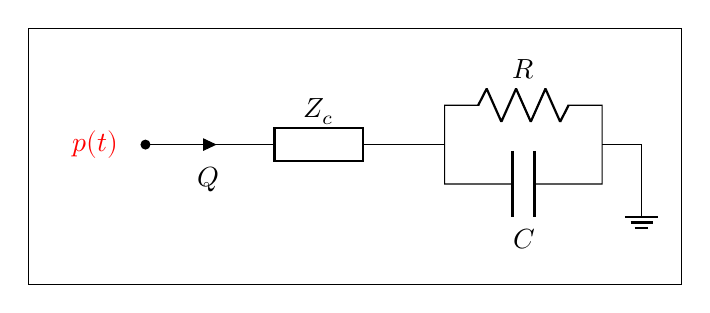
\begin{tikzpicture}
\node[draw, inner sep=8pt] {
    \begin{circuitikz}
    \draw (-.8,0) node[circ,label=left:$\color{red}p(t)$]{} to [short, i_=$Q$](.8,0) to [generic, l=$Z_{c}$](2,0) -- (3,0);
    \draw (3,0) -- (3,0.5) to[resistor, R=$R$] (5,0.5) -- (5,0);
    \draw (3,0) -- (3,-0.5) to[capacitor, l_=$C$] (5,-0.5) -- (5,0);
    \draw (5,0) -- (5.5,0) -- (5.5,-0.5) node[ground]{};
    \end{circuitikz}
};
\end{tikzpicture}
\end{center}
\end{minipage}
\hfill
\begin{minipage}{0.5\textwidth}
\textbf{Governing Equation:}
\[
    \frac{\mathrm{d} p(t)}{\mathrm{d} t}
    + \frac{p(t)}{RC} 
    = \frac{Q}{C} \bigg(1+\frac{Z_{c}}{R}\bigg) 
    + Z_{c} \frac{\mathrm{d} Q} {\mathrm{d} t}
\]
where $Z_{c}$ is the characteristic impedance, which denotes the resistance of the proximal vessel.
\end{minipage}

\paragraph{Four-element Windkessel Model} An inductor component, $L$, is introduced to account for the frequency-dependent relationship between pressure and flow, thereby representing blood inertance and capturing variations in arterial pressure response with changes in heart rate. \\

\begin{minipage}{0.5\textwidth}
\begin{center}
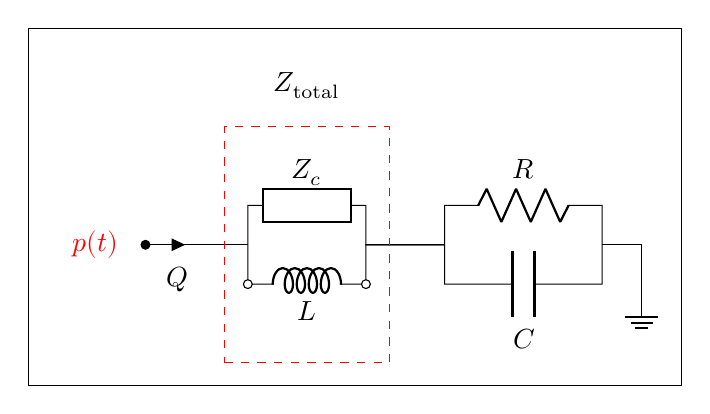
\begin{tikzpicture}
\node[draw, inner sep=8pt] {
    \begin{circuitikz}
    \draw (-.8,0) node[circ,label=left:$\color{red}p(t)$]{} to [short, i_={$Q$}](0,0) -- (.5,0);
    \draw (.5,0) -- (.5,0.5) to [generic, l=$Z_{c}$](2,0.5) -- (2,0) -- (3,0);
    \draw(.5,0) -- (.5,-0.5) to [inductor, l_=$L$, o-o](2,-0.5)-- (2,0) -- (3,0);
    \draw [red, dashed] (.2, -1.5) -- (2.3, -1.5) -- (2.3, 1.5) -- (.2, 1.5) -- cycle;
    \node[above=2pt] at (1.25,1.5) {$Z_{\mathrm{total}}$};
    \draw (3,0) -- (3,0.5) to[resistor, R=$R$] (5,0.5) -- (5,0);
    \draw (3,0) -- (3,-0.5) to[capacitor, l_=$C$] (5,-0.5) -- (5,0);
    \draw (5,0) -- (5.5,0) -- (5.5,-0.5) node[ground]{};
    \end{circuitikz}
};
\end{tikzpicture}
\end{center}
\end{minipage}
\hfill
\begin{minipage}{0.5\textwidth}
\textbf{Governing Equation:}
\[
    \frac{\mathrm{d} p}{\mathrm{d} t}
    + \frac{p(t)}{RC} 
    = \frac{Q}{C} \bigg(1+\frac{Z_{\rm{total}}}{R} \bigg)
    + Z_{\rm{total}}\frac{\mathrm{d} Q}{\mathrm{d} t}
\]
where $\displaystyle Z_{\rm{total}} = \frac{j\omega L Z_{c}}{j\omega L + Z_{c}}$ is the total impedance of the parallel network - the characteristic impedance, $Z_{c}$ and the inductor, $L$. 
\end{minipage}


\section{Moens-Korteweg Model of Pulse Wave Velocity}

\paragraph{Pulse waves} Blood is ejected into the aorta, generating a rapidly propagating wave of pressure (NOT flow!) accompanied by deformation of the aortic wall. This wave, also known as the \textbf{pulse wave}, travels along the arteries with a much faster speed (by orders of magnitude) than the bulk motion of blood, and undergoes reflections at sites of impedance mismatch such as arterial bifurcations.\\

The velocity of the pulse wave can be approximated by the Moens-Korteweg model:
\begin{equation*}
     {\rm PWV} = \sqrt{\frac{Eh}{2R\rho}},
\end{equation*}
where $E$ denotes the linear elasticity of the aortic wall, $h$ and $R$ are the wall thickness and wall radius, respectively, where $h \ll R$; and $\rho$ is the density of the blood. The Moens-Korteweg equation assumes blood is inviscid. \\

By definition, $\mathrm{PWV}$ increases with the stiffness of the vessels and decreases with the radius of the vessel.

\begin{figure}[H]
    \centering
    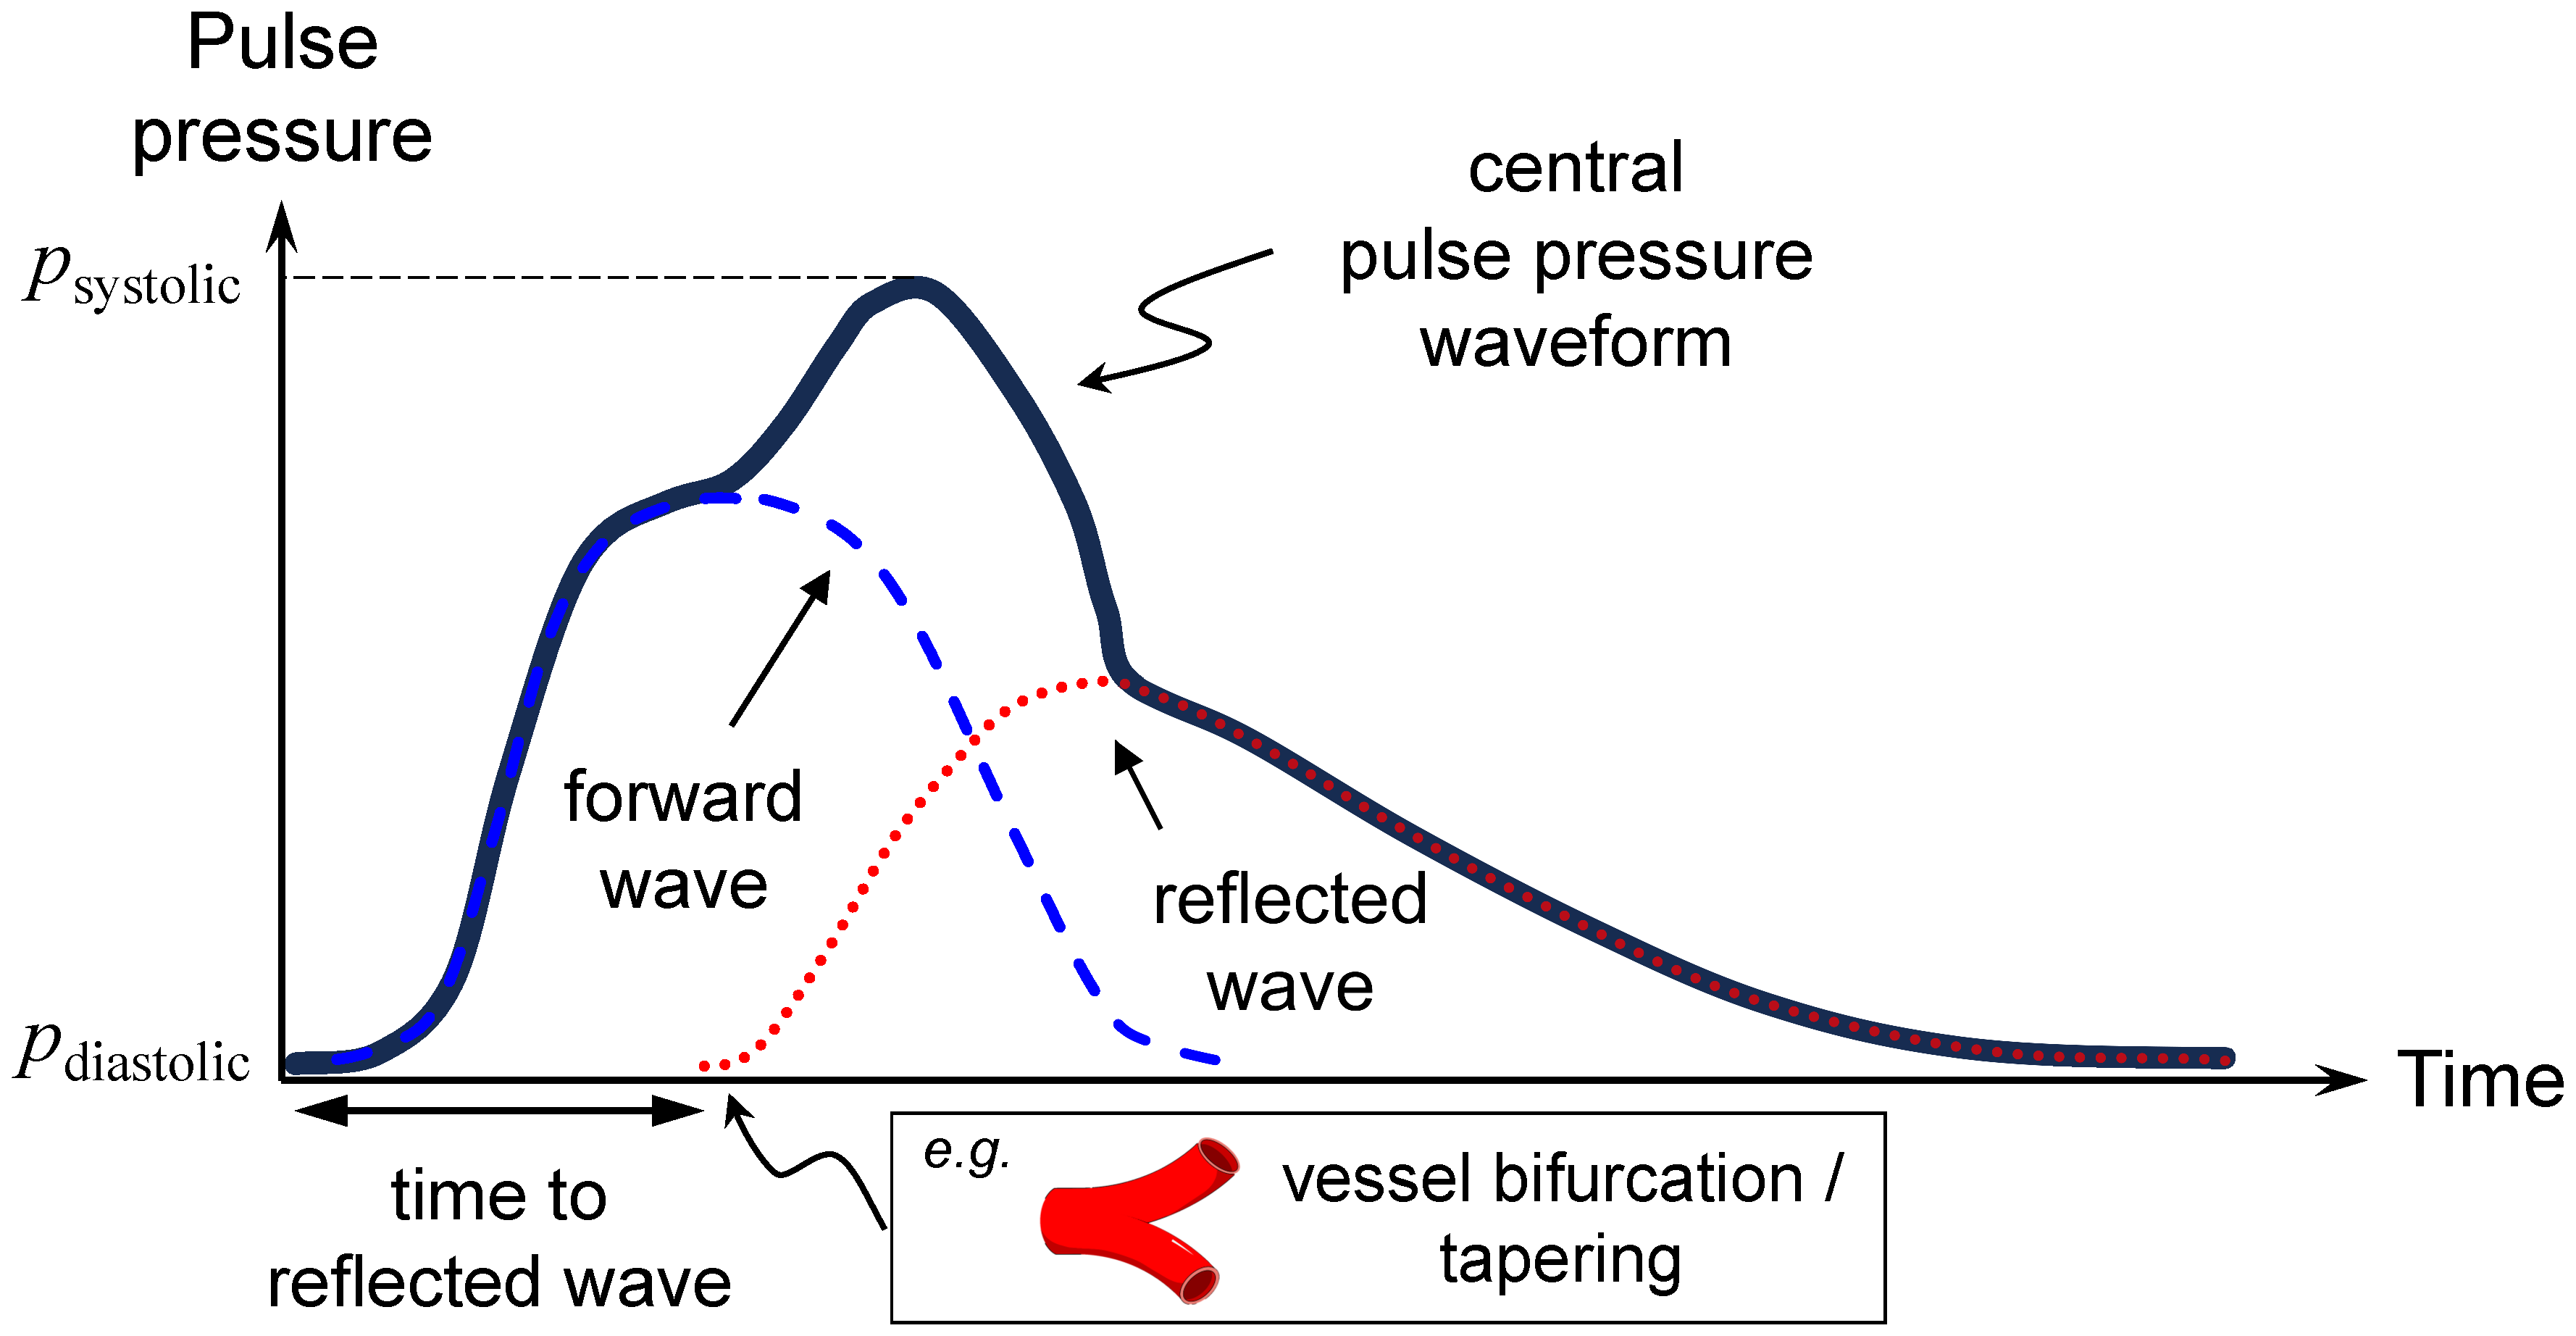
\includegraphics[width=.6\textwidth]{img/pulse_wave.eps}
    \caption{Schematic of the formation of the central arterial pressure waveform.}
\end{figure}


\vfill
{\small \color{gray}Drafted by B.~Li, with input from C.~H.~Yap, \today.}
%% TITLE	Physiological Fluid Mechanics, last page

%% DATE		- Nov 19, 2023     create

%% AUTHOR	BINGHUAN W LI (Dept. Chemical Eng/Bio Eng, Imperial)
%%          PETER Y XIE (Dept. Mech Eng, Stanford)

%% compiled in XeLaTeX with Tex Live version 2023.

%% This work is licensed under a Creative Commons Attribution-NonCommercial 4.0 International License.

\newpage
\thispagestyle{empty}
\newgeometry{margin=1.8cm}

\mbox{}
\vfill    
\begin{figure}[H]
    \includegraphics[right]{img/by-nc.eps}
\end{figure}
\textit{This work is licensed under a Creative Commons Attribution-NonCommercial 4.0 International License.}

\end{document}